\chapter{Análisis de Efectividad de los Oráculos}

En esta sección, se presenta el diseño del experimento realizado para evaluar la efectividad de los oráculos generados automáticamente. También se presentan los resultados obtenidos.

\section{Evaluación Experimental}

Se describe el diseño del experimento y cómo se evaluaron los oráculos generados.

\subsection{Generación de oráculos}

Para comparar la eficiencia de pruebas de regresión generadas con distintos enfoques, aserciones de test y contratos se plantean los siguientes pasos. 

Dado un código que representa una solución correcta a un problema específico, como primer paso se deben generar casos de pruebas utilizando las herramientas de generación automática mencionadas en el Capítulo 2.

1) Generación de tests utilizando Randoop.
A partir del archivo ejecutable del código bajo prueba, la clase y el método a probar. Obtendremos aserciones como hemos visto en el Código 2.2 de la sección 2.4.1.


\begin{lstlisting}[style=bashstyle, caption=Generación de tests con Randoop, label=lst:bashcode]
java -cp ${randoop_jar}:${project_classpath} randoop.main.Main gentests $test_classes --classlist=$classlist --serialize-folder=$mutator_inputs --serialize-method=\"$regex_method\" --junit-package-name=$package --junit-output-dir=$outdir_tests --junit-reflection-allowed=false --time-limit=$timelimit --literals-level=ALL --literals-file=$literals --omit-methods=\"$omitmethods\"
\end{lstlisting}


2) Generación de aserciones utilizando Daikon. 
A partir de los archivos ejecutables de las pruebas generadas con Randoop, el código bajo prueba, el nombre de la clase y el método a probar, al ejecutar el siguiente script se obtienen aserciones Daikon como se ha visto en el Código 2.3 de la sección 2.4.2.

\begin{lstlisting}[style=bashstyle, caption=Generación de tests con Randoop, label=lst:bashcode]
# First step: perform dynamic comparability analysis (with DynComp)
java -cp \
 ${tests_bin}:${daikon_path}/daikon.jar:${subject_jar} \
 daikon.DynComp --output-dir=${output_dir}daikon/ \
 ${package}.RegressionTestDriver

# Second step: obtain the dtrace file with Chicory
echo '--> Going to run Chicory'
java -cp \
 ${tests_bin}:${daikon_path}/daikon.jar:${subject_jar} \
 daikon.Chicory --comparability-file=\
 ${output_dir}daikon/RegressionTestDriver.decls-DynComp \
 --output-dir=${output_dir}daikon/ ${package}.RegressionTestDriver

# Third step: actual Daikon execution to infer specs
echo '--> Going to run Daikon'
java -cp ${daikon_path}/daikon.jar daikon.Daikon \
 --ppt-select-pattern \
 ${package}'\.'$2':::CLASS|'${package}'\.'$2':::OBJECT|\
 '${package}'\.'$2'\.'$method_without_args \
 -o ${output_dir}daikon/res.inv.gz \
 ${output_dir}daikon/RegressionTestDriver.dtrace.gz

# Process result and print the Daikon specs for better readability. First
# the ones related to class invariants, and then the ones related to the current method
java -cp ${daikon_path}/daikon.jar daikon.PrintInvariants \
 ${output_dir}daikon/res.inv.gz --format java > ${output_dir}daikon/res.txt
\end{lstlisting}


3) Generación y compilación de mutantes utilizando Major.

\begin{lstlisting}[style=bashstyle, caption=Generación de mutantes con Major, label=lst:bashcode]
$major/bin/javac -cp $subject_jar -nowarn -J-Dmajor.export.mutants=true -XMutator:ALL \
 -d ${output_dir}bin ${source_dir}src/main/java/$class_path/${2}.java
\end{lstlisting}


4) Ejecución de las aserciones generadas por Randoop sobre cada mutante.
Para cada ejecución se analiza la salida, básicamente puede obtenerse como resultado que las aserciones no encuentran errores o por el contrario si lo encuentran, es decir que detectan la mutación. En este último caso, a su vez es necesario identificar aquellas ejecuciones en las que las aserciones fallan, de las que son ejecuciones erroneas.
En la siguiente tabla se puede visualizar un ejemplo del resultado obtenido.

\vspace{10pt}

\csvautotabular{stackAr-top-randoop-result.csv}

\vspace{10pt}

5) Ejecución de las aserciones generadas por Daikon sobre cada mutante. En la siguiente tabla se pueden ver los resultados obtenidos para el ejemplo.

\vspace{10pt}

\csvautotabular{stackAr-top-daikon-result.csv}

\vspace{10pt}


\section{Resultados}

Se presentan los resultados obtenidos en el experimento y se analizan.

\begin{figure}[ht]
\centering
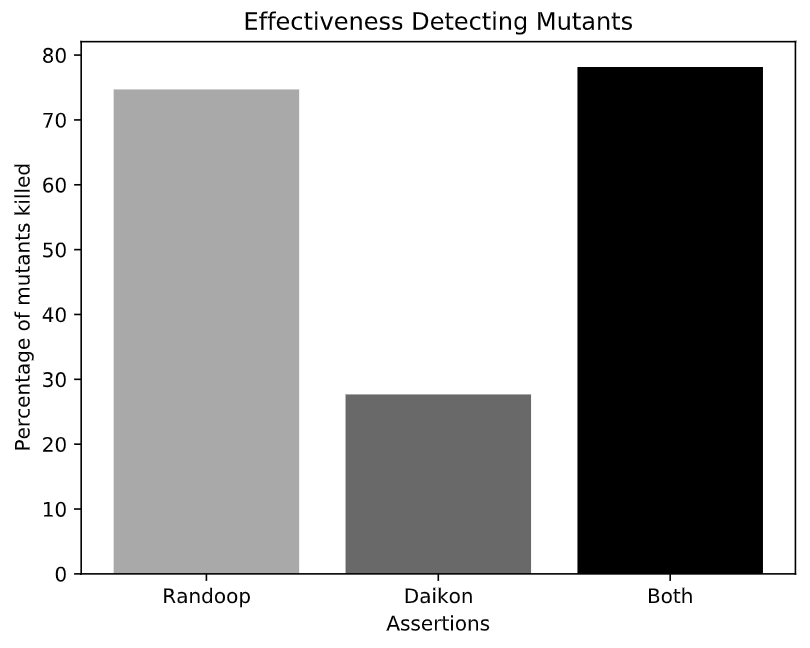
\includegraphics[width=0.8\textwidth]{tools-effectiveness.png}
\caption{Resultados obtenidos}
\label{fig:nombre_etiqueta}
\end{figure}

\vspace{10pt}

\csvautotabular{effectiveness.csv}

\vspace{10pt}



Graficos y Tablas segun mutante

\vspace{10pt}

\csvautotabular{effectiveness-by-mutant-type.csv}

\vspace{10pt}


Se puede observar de los resultados obtenidos que las aserciones generadas por Randoop detectaron el 74.7\%, mientras que Daikon detectó el 27.67\%. 

El total de aserciones generadas por Randoop es de 31030.
Mientras que Daikon generó 5648 contratos.

Algunos casos particulares donde Daikon supera a Randoop.
SimpleMethods_incrementNumberAtIndex
Composite.addChild (detecta distintos casos)
listcomp02_insert_s
BooleanUtils.toBoolean
public static boolean toBoolean(final Integer value, final Integer trueValue, final Integer falseValue) {
  boolean result = false;
  if (value == null) {
    if (trueValue == null) {
        result = true;
    } else if (falseValue == null) {
        result = false;
    }
  } else if (value.equals(trueValue)) {
      result = true;
  } else if (value.equals(falseValue)) {
      result = false;
  } else {
    // no match
    throw new IllegalArgumentException("The Integer did not match either specified value");
  }
  assert (true);
  return result;
}


Randoop con 2203 aserciones detectó 4 de 18 mutantes.
Mientras que Daikon detectó 16 de 18 mutantes.

Contrato generado por daikon
===========================================================================
lang3.BooleanUtils.toBoolean(java.lang.Integer, java.lang.Integer, java.lang.Integer):::ENTER
value == falseValue
value != null
trueValue != null
===========================================================================
lang3.BooleanUtils.toBoolean(java.lang.Integer, java.lang.Integer, java.lang.Integer):::EXIT
\result == false


Mutantes:
1:LVR:51:false |==> true
2:ROR:52:value == null |==> false
3:ROR:53:trueValue == null |==> false
4:LVR:54:true |==> false
5:STD:54:result = true |==> <NO-OP>
6:ROR:55:falseValue == null |==> false
7:LVR:56:false |==> true
8:STD:56:result = false |==> <NO-OP>
9:COR:58:value.equals(trueValue) |==> false
10:COR:58:value.equals(trueValue) |==> true
11:LVR:59:true |==> false
12:STD:59:result = true |==> <NO-OP>
13:COR:60:value.equals(falseValue) |==> false
14:COR:60:value.equals(falseValue) |==> true
15:LVR:61:false |==> true
16:STD:61:result = false |==> <NO-OP>
17:LVR:66:true |==> false
18:EVR:67:result |==> false

Randoop detectó mutantes 2, 6 y 7.
Daikon no detectó 5 y 9 
